% \documentclass[10pt,twocolumn,letterpaper]{article}
\documentclass[10pt,letterpaper]{article}
%% Welcome to Overleaf!
%% If this is your first time using LaTeX, it might be worth going through this brief presentation:
%% https://www.overleaf.com/latex/learn/free-online-introduction-to-latex-part-1

%% Researchers have been using LaTeX for decades to typeset their papers, producing beautiful, crisp documents in the process. By learning LaTeX, you are effectively following in their footsteps, and learning a highly valuable skill!

%% The \usepackage commands below can be thought of as analogous to importing libraries into Python, for instance. We've pre-formatted this for you, so you can skip right ahead to the title below.

%% Language and font encodings
\usepackage[spanish,english]{babel}
\usepackage[utf8x]{inputenc}
\usepackage[T1]{fontenc}

%% Sets page size and margins
\usepackage[a4paper,top=1.5cm,bottom=1.5cm,left=1.5cm,right=1.5cm,marginparwidth=1.75cm]{geometry}
\setlength{\parskip}{0.3\baselineskip}
% \setlength{\parindent}{0pt}

%% Useful packages
\usepackage{amsmath}
\usepackage{graphicx}
\usepackage[colorinlistoftodos]{todonotes}
\usepackage[colorlinks=true, allcolors=blue]{hyperref}
\usepackage{enumitem} 

% \setlist{nosep, itemsep=5pt, parsep=0pt, before={\parskip=0pt}, after=\vspace{-\parskip}}%
\setlist{nosep, itemsep=3pt, parsep=0pt}%

\graphicspath{{images/}}

%% Title
\title{
		%\vspace{-1in} 	
		\usefont{OT1}{bch}{b}{n}
		% \normalfont \normalsize \textsc{STEM Fellowship Journal Template} \\ [14pt]
		\huge HTML2023 Spring Final Project \\
}

\usepackage{authblk}

\author{b10902003, b10902067}
% \author[1]{Third Author}
% \author[1,3]{Fourth Author}

	% \affil[1]{\small{CSIE, National Taiwan University}}
% \affil[2]{Department, Institution/School}
% \affil[3]{Department, Institution/School} 


\begin{document}
\maketitle

\selectlanguage{english}
% \begin{abstract}
% The abstract is in a sense the most important part of your paper, since many readers will scan an abstract first before deciding to invest effort in reading the paper.

% An abstract should be about 300 words long at most, and should act as a clear summary of the paper. It should state the aim and scope of the research, methods, results and conclusions, and the implications of the paper’s finding. The abstract should be broadly accessible (i.e. able to be understood by as many people as possible - even those outside the field) and communicate the importance of the work being done. 

% Structure the abstract as follows: background and aims, methods, results and conclusion. Please note that review articles will not contain methods or results. 

% Examples of ideal abstracts can be found \href{http://journal.stemfellowship.org/userimages/ContentEditor/1451371646443/AbstractExamples.pdf}{here}, with the main ideas highlighted.
% \end{abstract} 

% \section*{Keywords}
% Select keywords with care, because they will help users discover your paper. To determine appropriate keywords, put yourself in the position of someone who is trying to search for a paper like yours. What search terms would you use? From those terms, select a list of at least three and no more than five words. Include these words in the text of the abstract and if at all possible, in the title of the paper.

\section{Initial Settings}
\subsection{Data Inspection}

The features in the dataset can be classified into three types:
\begin{itemize}
  \item Ordinal: \texttt{Energy, Key, Loudness, Speechiness, Acousticness, Instrumentalness, Liveness, Valence, Tempo, Duration\_ms, Views, Likes, Comments}
  \item Categorical: \texttt{Album\_type, Licensed, official\_video, Album, Channel, Composer, Artist}
  \item Text: \texttt{Track, Uri, Uri\_spotify, Url\_youtube, Description, Title}
\end{itemize}

Notice that we drop ID since it is a manually added feature in the dataset, it should provide no insight about the danceability of each track. We also drop text data, due to the fact that it is provided by the uploader and has no standardized format. We believe that in such cases, it contains more noise than the insight about danceability. 

Diving into the dataset, we found out that there are only 11 composers and 97 artists. It seemed unnatural to us that there are such less unique composers and artists given that we have more than 17,000 tracks. We dug into several tracks and realized that both features are totally incorrect, and provide us nothing but misleading information. As a result, we also dropped those two features.

We also observed that there are some uncanny information in the testing dataset. For example, negative values in \verb|Duration_ms| and decimals in \verb|Views|! Those information appear after \verb|id=19170|, which is the 2001-th test data. Moreover, aside from unreasonable values, some features (e.g. Loudness, Speechiness, etc.) have over 10 decimal places after the 2001-th test data and only 3 decimal places before. In light of those weirdness, we made a assumption that \textbf{Nijika} had fiddled those test data. To counter such mischief, we had different approaches toward the two sections of data. For the first 2000 test data, we believe they are more related to the training data and thus apply models with stronger power and less regulizations; as for the remaining data, we believe there are huge amounts of noise and thus apply stronger regulization on the models. 

In conclusion, we mainly focus on the ordinal features. Inside each model, the feature selection is performed manually by permuation test or automatically by the model (e.g. ShapValues in CatBoost). The details are specified in each model subsection. 

\subsection{Combat Missing Values}

We have observed that 15\% of the data is missing in each feature.
In order to facilitate the use of commonly employed machine learning models, 
it is necessary to fill in these missing portions with appropriate data. 
Firstly, we need to determine whether the missing data is randomly selected. 
In some features, such as Channel, where it is relatively easier to obtain the original data, 
we have found that the missing data is likely to be randomly selected. 
Based on our belief that the missing data is randomly selected, 
we have chosen to use mean and median imputation to fill in the missing values, 
without further exploring whether alternative approaches would yield better performance.

\subsection{Validation Dataset}

In the first stage, we use k-fold cross validation to tune the parameters and evaluate each model. Nonetheless, the public score is quite far away from the validation score. As we could see in Figure~\ref{fig:EvalEpublicScatter}, the public score is roughly $0.2$ higher than validation score. When the public score is around $1.9$, we can barely tell which model is better according to the validation score. It felt like the public score was randomly hovering around $1.9$. We believe that this is due to the manual distortion in test data and thus the validation score can only provide a considerably vague approximation on the public / private score.

\begin{figure}[h]
	\centering
	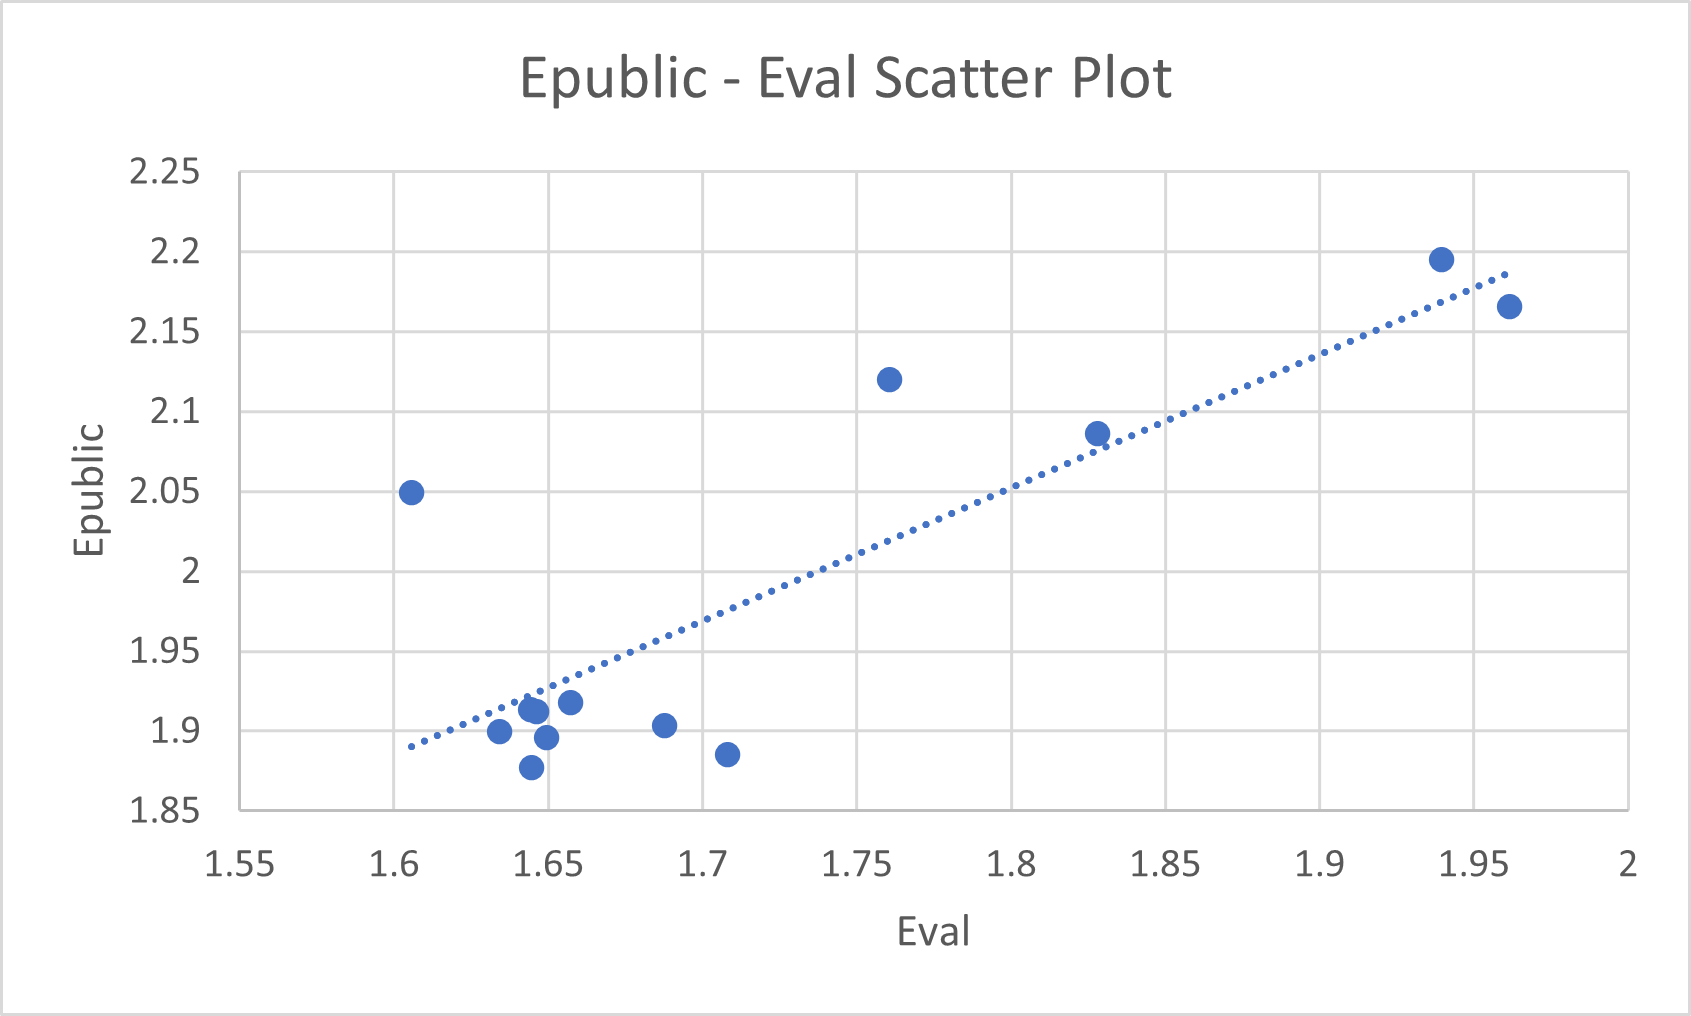
\includegraphics[width=0.4\textwidth]{Eval-Epublic-scatter.png}
	\caption{The scatter plot of Eval and Epublic with linear regression line}
	\label{fig:EvalEpublicScatter}
\end{figure}

Blindly follow the validation score seemed to lead to an overfitting on the training dataset, and did not help us much on selecting the best model. Therefore, we utilized the 5 submissions per day to try out every possible model we had, and managed to reach a relatively lower public score by the end of the first competition. However, on the award ceremony, professor Lin revealed that there is a distribution shift between public and private dataset. Thus what we had done was overfitting on the public dataset, resulting in an appalling private score. 

In the second stage, we are given a small subset of the private dataset. Considering the problematic validation score above, we decided to apply it on validating and give up on cross validation. We believed that we had had enough training data but lack in validating, thus apply it on validation may make the greatest use on it. 

% During the first stage award ceremony, our team had won the third prize in private score and were blessed with a glance in the private score of a specific submission. 

\section{Individual Models}

In this section, we discuss three main models which performed the best in predicting \texttt{Danceability}. Other models that we had tried but did not performed well are discussed in the last subsection. 

\subsection{Support Vector Regression}

Support Vector Regression (SVR) is our first model that passed the baseline. We opted to study this model first because we are familiar with it and it provides good method to combat overfitting. Ultimately, it reached a score of $2.084$ in the validation dataset, which was the second-best performance among all individual models. 

\subsubsection{Setup}
\begin{itemize}
	\item Package: LIBSVM
	\item Selected Features: \texttt{Instrumentalness, Speechiness, Energy, Valence, Acousticness, Liveness, Tempo, Key, Composer}
	\item Parameters: \texttt{-s 3 -t 2 -c 0.01 -g 0.5 -e 0.00001 -h 0}
\end{itemize}

\subsubsection{Introduction}

SVR extends the idea of one class Support Vector Machine (SVM). The only difference is that we have $y_i \in \{0, 1, \dots, 9\}$ instead of $y_i \in \{-1, 1\}$. The minimizing target is basically identical
$$
	\frac{1}{N} \sum \lvert \mathbf{w}^t \mathbf{x_i} + b - y_i \rvert
$$
Yet, to adapt the new $y_i$, LIBSVM provide a new minimize problem
\begin{align*}
	\underset{\mathbf{w}, b, \mathbf{\xi}, \mathbf{\xi^*}}{\min} \quad & \frac{1}{2}\mathbf{w}^T\mathbf{w} + C\left(\sum_{i=1}^m \xi_i + \sum_{i=1}^m \xi^*_i\right) \\
	\text{subject to} \quad & (\mathbf{w}^T \mathbf{x} + b) - y_i \le \epsilon + \xi_i \\
	& y_i - (\mathbf{w}^T \mathbf{x} + b) \le \epsilon + \xi^*_i \\
	& \xi_i, \xi^*_i \ge 0
\end{align*}
By tuning $C$, we may set the importance of regularizer; tuning $\epsilon$, we may set the tolerable error. It also supports kernel trick like regular SVM by setting \texttt{-t} and \texttt{-g} parameters. 

\subsubsection{Preprocessing}

While playing around with the SVR, we observed that the model is highly sensitive to the scale of each feature. This is an expected phenomenon since SVM also suffers from it, a larger scale may result in a smaller $w_i$, which ruins the regularizer. Given that some features have quite different distributions between training and testing datasets, we selected features which have similar scaling in both training and testing datasets, and rescaled the range of each feature to unit size in order to combat the scaling issue. 

There are data that exhibited excessive concentration around $0$, such concentration will also result in a larger $w_i$. We applied some non-linear transformations (e.g. square root) to disperse their distributions to combat it. As for categorical features, we attempted one-hot encoding on \texttt{Composer} and \texttt{Artist}, which were deemed more likely to be related to \texttt{Danceability} in terms of their physical meanings. Nonetheless, we found that while the inclusion of \texttt{Artist} decreased training error (Ein), it marginally increased both cross-validation error (Ecv) and public score. Consequently, we dropped the \texttt{Artist} feature.

\subsubsection{Parameters}

During the first stage, we tuned the parameters according to cross-validation error (Ecv). We selected \texttt{-t 2 -c 10 -g 0.5 -e 0.00001} as the best parameters, which represents 
\begin{align*}
	\underset{\mathbf{w}, b, \mathbf{\xi}, \mathbf{\xi^*}}{\min} \quad & \frac{1}{2}\mathbf{w}^T\mathbf{w} + 10\left(\sum_{i=1}^m \xi_i + \sum_{i=1}^m \xi^*_i\right) \\
	\text{subject to} \quad & (\mathbf{w}^T \mathbf{\Phi(x)} + b) - y_i \le 0.00001 + \xi_i \\
	& y_i - (\mathbf{w}^T \mathbf{\Phi(x)} + b) \le 0.00001 + \xi^*_i \\
	& \xi_i, \xi^*_i \ge 0
\end{align*}
with kernel function
$$
	K(\mathbf{x}, \mathbf{x'}) = \exp(-0.5 \lvert \mathbf{x} - \mathbf{x'}\rvert^2)
$$
The model reached $\text{Ein} = 1.60594, \text{Ecv} = 1.68433, \text{Epublic} = 1.88533$. 

In the second stage, we tuned the parameters again, but instead refer to the validation dataset (Eval). We selected \texttt{-t 2 -c 0.01 -g 0.5 -e 0.00001} as the best parameters, which represents
\begin{align*}
	\underset{\mathbf{w}, b, \mathbf{\xi}, \mathbf{\xi^*}}{\min} \quad & \frac{1}{2}\mathbf{w}^T\mathbf{w} + 0.01\left(\sum_{i=1}^m \xi_i + \sum_{i=1}^m \xi^*_i\right) \\
	\text{subject to} \quad & (\mathbf{w}^T \mathbf{\Phi(x)} + b) - y_i \le 0.00001 + \xi_i \\
	& y_i - (\mathbf{w}^T \mathbf{\Phi(x)} + b) \le 0.00001 + \xi^*_i \\
	& \xi_i, \xi^*_i \ge 0
\end{align*}
with kernel function
$$
	K(\mathbf{x}, \mathbf{x'}) = \exp(-0.5 \lvert \mathbf{x} - \mathbf{x'}\rvert^2)
$$
The model reached $\text{Ein} = 2.01934, \text{Eval} = 2.07765, \text{Epublic} = 2.0643$. 

The first set of parameters had lower errors, which lured us to select it as the final parameters. However, due to the distribution shift between public and private dataset, the second set seemed to be a more generalized and robust approach. As we can see in the errors, Eval approximated Epublic better, which made us believe that it also approximates Eprivate well. In addition, the only difference between the two sets is the regularizing weight ($C$). The first set emphasized more on the error itself while the second penalized more on model complexity. We believed that given Ein is much lower than Epublic, we had had enough model power but lack in regularization. Therefore, we selected the second set as the final parameters of SVR. 

% \subsubsection{Results}
% The model is relatively slow with such large dataset. On average, a training and predicting process requires $19.7$ seconds with around $650\%$ CPU usage. 

\subsection{Stochastic Gradient Descent Regressor}

The second model is stochastic gradient descent regressor (SGD Regressor). This is similar to SVR but approaches the minimum by a stochastic method, resulting in a more efficient, robust and generalized model.

\subsubsection{Setup}
\begin{itemize}
	\item Package: scikit-learn (\verb|sklearn.linear_model.SGDRegressor|)
	\item Selected Features: ordinal + categorical
	\item Parameters:\begin{itemize}
		\item RFE: \verb|n_features_to_select=42, step=1|
		\item SGDRegressor: \texttt{loss='epsilon\_insensitive', epsilon=0.08, penalty='l2', alpha=1.2e-6, max\_iter=1000, tol=0.06, shuffle=True, random\_state=0xCC12}
	\end{itemize}
\end{itemize}

\subsubsection{Introduction}

SGD Regressor aims to solve a problem similar to SVR, it minimizes the following penalized error
$$
	E(\mathbf{w}, \mathbf{b}) = \frac{1}{n}\sum_{i=1}^n L(y_i, f(\mathbf{x_i})) + \alpha R(\mathbf{w})
$$
Yet, SGD Regressor and SVR differs in the method of approaching minimum. SGD regressor descents according to a randomly selected subset of data during each iteration, giving it the "stochastic" name. 

By setting the loss function to epsilon-insensitive, we can match the \textbf{Nijika}'s target error (MAE)
$$
	L(y_i, f(\mathbf{x_i})) = \max(0, \lvert y_i - f(\mathbf{x_i})\rvert - \epsilon)
$$
$\epsilon$ represents the tolerable error, $\alpha$ represents the importance of regularizer and a hidden parameter \texttt{tol} indicates the stopping criterion. 

\subsubsection{Preprocessing}

\begin{figure}[h]
	\centering
	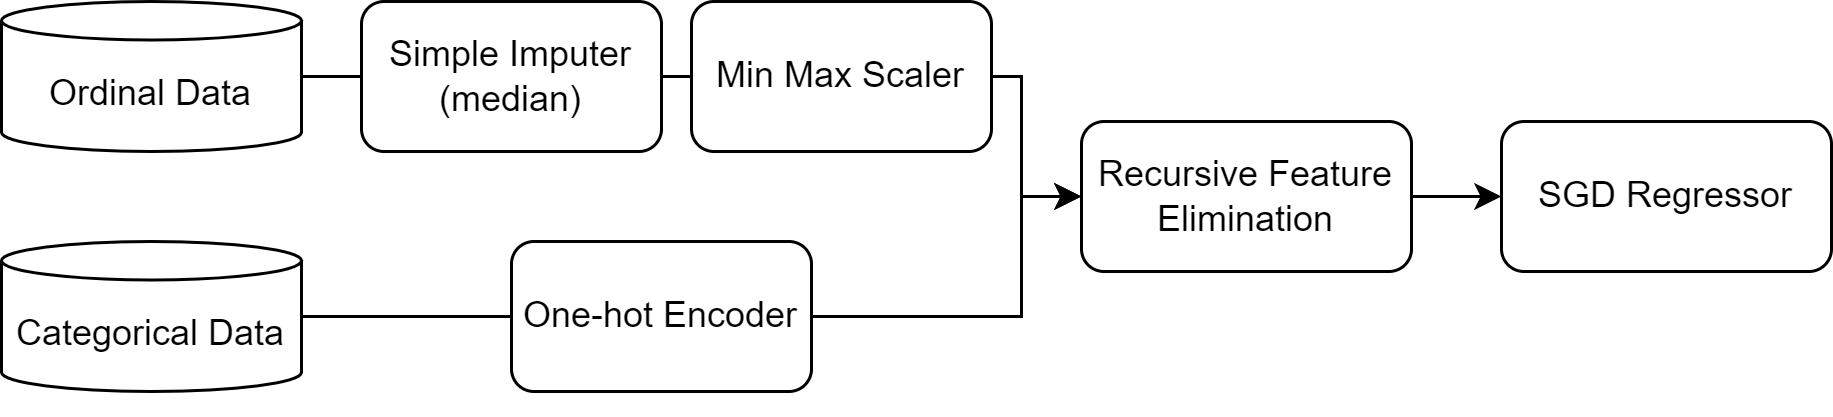
\includegraphics[width=0.6\textwidth]{SGDregressor-diagram.png}
	\caption{The preprocessing diagram of SGD Regressor}
	\label{fig:SGDRegressorDiagram}
\end{figure}

Since SGD Regressor is also sensitive to feature scaling, we had to apply scaling to the ordinal features. In SGD regressor, we tried several scaler and found out that \texttt{sklearn.preprocessing.MinMaxScaler}, scaling values to unit length, outperformed the rest. We believed that this is because one-hot encoder transforms categorical features to $0$ or $1$, having the other features scaling to $[0, 1]$ will best fit the regularizer. 

We also tried polynomial transformation on the dataset. Though it decreases Ein, the validation score was horrible. Apparently, applying polynomial transformation had given too much power on the model and thus overfitted on the training dataset. 

Aside from those transformations, we also applied feature selection on the transformed features. We utilized \texttt{sklearn.feature\_selection.RFE} to complete the task. It performed a recursive feature elimination, removing the least important feature on each iteration according to its coefficient calculated by the regressor model. We believed that it not only reduced computation time, but also improved generality. As a result, Eval decreased from $2.06367$ to $2.05658$, making a slight improvement. 

\subsubsection{Parameters}

In this model, we tuned four parameters: $\epsilon, \alpha$, \texttt{tol}, \texttt{n\_features\_to\_select}, according to Eval.
The best set was $\epsilon=0.08, \alpha=0.0000012$, \texttt{tol}$=0.06$, \texttt{n\_features\_to\_select}$=42$, which gave an Eval of $2.05658$. The corresponding error function is 
$$
	E(\mathbf{w}, \mathbf{b}) = \frac{1}{n}\sum_{i=1}^n \max(0, \lvert y_i - f(\mathbf{x_i})\rvert - 0.08) + 0.00000012\lVert\mathbf{w}\rVert^2
$$

\subsection{Cat Boost}

Our third model is Cat Boost. It achieved a score of $2.111$ on the validation dataset, representing the best-performing tree model prior to the submission deadline. 

\subsubsection{Setup}

\begin{enumerate}
	\item Package: CatBoost
	\item Selected Features: \texttt{Instrumentalness, Speechiness, Energy, Valence, Acousticness, Liveness, Tempo, Key, Composer, Artist}
	\item Parameters: \verb|CatBoostRegressor(task_type="GPU", devices='0', random_state=0xCC12, loss_function='MAE',|\linebreak
						\verb|eval_metric = 'MAE', cat_features=[Composer, Artist]).select_features(eval_set=[released data],|\linebreak
						\verb|features_for_select='0-9', num_features_to_select=8,|\linebreak
						\verb|algorithm=EFeaturesSelectionAlgorithm.RecursiveByShapValues,|\linebreak
						\verb|shap_calc_type=EShapCalcType.Regular,train_final_model=True)|
\end{enumerate}

\subsubsection{Introduction}

CatBoost is an optimized version of Gradient Boosting Trees, offering additional functionalities such as categorical feature support, a fast GPU version, and good results with default parameters. Therefore, in the introductory section, we focus on the Gradient Boosting Tree (regression) algorithm itself.

Regressor Tree is based on the Decision Tree, with the difference being that the categories at each node represent the predicted values of y instead of class labels. When determining the predicted value at a node, the algorithm optimizes the loss function for the training data at that node. During the branching process, the algorithm compares features in a way that maximally separates the training data with different ranges of y values.

Gradient Boosting involves training subsequent models to predict the difference between the y value and the sum of the predictions from all previous models. This approach allows weak learners to combine and form a strong model. When the loss function permits, efficient computations can be performed using differentiation.

In summary, Gradient Boosting Tree utilizes Regressor Tree for the purpose of Gradient Boosting. Therefore, we can use model parameters related to trees or limit the number of training iterations in Gradient Boosting to combat overfitting.

\subsubsection{Preprocessing}

We selected the better preprocessing method from the two methods we already implemented, rather than developing a new one. We utilized the method described in the SVM section, which was chosen based on error metrics.

\subsubsection{Parameters}

We employed two additional methods to enhance our model. The first method involved constraining the tree depth and applying l2 regularization at the leaf nodes. The second method was utilizing a built-in feature selection tool. We found that the approach utilizing feature selection exhibited better performance on the released dataset, leading us to adopt the feature selection version as our final choice.

% CatBoost is an optimized version of Gradient Boosting Trees. It natively supports categorical features and allows the inclusion of a validation dataset to retain the best iteration, thereby reducing the need for parameter tuning while mitigating overfitting. We utilized the similar input as SVR and employed two additional methods to enhance our model. The first method involved constraining the tree depth and applying l2 regularization at the leaf nodes. The second method was utilizing a built-in feature selection tool. We found that the approach utilizing feature selection exhibited better performance on the released dataset, leading us to adopt the feature selection version as our final choice.

\subsection{Other Models}

In addition to the aforementioned models, we also experimented with various models such as neural networks and random forests. However, their performance on the public score and validation dataset fell short of the three models above. Hence, we excluded them from the final selection.

Furthermore, we discovered that several linear models, such as BayesianRidge, ARDRegression, ElasticNetCV, LassoLarsCV, as well as neural networks that only utilized linear activation achieved scores around $2.13$ on the validation dataset. These models demonstrated favorable performance after fine-tuning, but due to the limitations in time, we had chosen to focus on the three models above which gave the best performance. 

\section{Blending}

In the final stage, we merged the aforementioned models that yielded satisfactory results into a single model. 
As we had exhausted all available datasets during the training of the preceding models, 
to prevent overfitting, we simply assigned different weights to each model based on our understanding of their performance. 
SVM and SGDRegressor exhibited the best performance, thus receiving higher weights, 
while the other models were assigned lower weights. 
We believe that such an allocation contributes to controlling the upper bound of the private score while providing opportunities for effective error correction. 
Through simple mathematical reasoning, 
it can be deduced that the worst-case scenario for the private score is the sum of each model's private score multiplied by their respective weights. 
Due to the higher weights assigned to SVM and SGDRegressor, the worst-case scenario for Blending does not deviate significantly from the performance of these two models. 
Simultaneously, when different models make predictions on the same value, 
if their predictions fall on opposite sides of the correct answer, 
we can anticipate improved results through the blending of predicted values.

Ultimately, this model achieved a score of $2.039$ on the released data, outperforming all individual models.

\section{Final Result}

\newpage

\bibliographystyle{vancouver}
\bibliography{references}

% \begin{thebibliography}{9}
% All information or data from other sources or authors must be appropriately cited at each point in the text where the source is relevant. All sources should be listed in a bibliographic reference section at the end of the paper with the heading "Reference List". 

% If the paper contains any copyright material, such as tables, figures, images, or other, the authors must obtain written permission from the copyright holder and provide it to the editor. 

% Bibliographic references should conform to the Vancouver style. In this style, bibliographic references are numbered and citations in the text to each reference should be numbers in square brackets; e.g., [1]. 

% If you are using a reference management system (such as Zotero, Mendeley or ReadCube), you may be able to export your bibliography as a Bib\TeX{} file. 

% Please refer to the comments in this template for how to format your references in LaTeX (either with a .bib file, or via manual input of references).


%% Please read the following comments for instructions on formatting your references.
%% The provided style file formats references in the required Vancouver style
%% This is a useful guide to formatting bibliographies using LaTeX (https://en.wikibooks.org/wiki/LaTeX/Bibliography_Management)

%% References with BibTeX database:
%%Bib\TeX{} is a bibliographic tool that is used with \LaTeX{} to help organize the user's references and create a bibliography. This short tutorial explains how to use BibTex files [https://www.latex-tutorial.com/tutorials/beginners/latex-bibtex/].

%%For references without a BibTeX database:
%%Your line of code will start with the \bibitem{cite_key} command. This is a unique identifier for a reference, such as #\bibitem{Lindquist95} or  #\bibitem{Smithetal2002}. Following the #\bibitem{cite_key} command is the actual reference. Here you should include all relevant details for the reference e.g. authors, title, year of publication, etc. The \bibliographystyle{vancouver} will format these references to the correct Vancouver style - as required by the STEM Fellowship Journal.

%% \bibitem must have the following form:
%%   \bibitem{key}...
%%

% \bibitem{}
% Below is an example.

%%\bibitem{Smithetal2002}

% \end{thebibliography}

\end{document}